For the sake of learning, the project is deployed to two different environments/setups. One using a VM created using Vagrant, and another AKS cluster hosted on Microsoft Azure platform.
\subsubsection{Virtual Machine created using Vagrant}      

\subsubsection*{Vagrant Deployment}
We use Vagrant with the plugins vagrant-azure and vagrant-docker-compose.

\noindent With vagrant-azure we configure a VM in Azure, specify which ports should be open, VM size, and similar details.

\noindent Once the VM is running Vagrant will do the following.
\begin{itemize}
\item Setup Docker.
\item Insert an ssh key as an authorized key, that will be used by our GitHub Actions workflow later.
\item Transfer the docker-compose.yml file
\item Use the vagrant-docker-compose plugin to setup Docker-compose, and start the app defined in docker-compose.yml
\end{itemize}

When Vagrant is finished setting up the VM, our MiniTwit app will be online.

\subsubsection{AKS cluster hosted on Azure}
Azure provides a production-ready configurable cluster as PaaS, and it was a perfect choice for the MiniTwit use case since it's a low budget project. Creating Kubernetes from scratch requires at least three VM of a specific type that match the Azure requirement for hosting the master node as well as for the worker node in the node pool. Since this project is running on a student’s subscription with limited credit, it was not affordable. However, the design for such a self-managed cluster requires a master node to run Kubernetes main functionalities including the API, a worker node to run pods inside which the docker container will run, a public client to be the proxy for interacting with the controller and managing the deployment flow, see Figure \ref{fig:k8sdiagram} % add picture.
\begin{figure}[H]
    \centering
    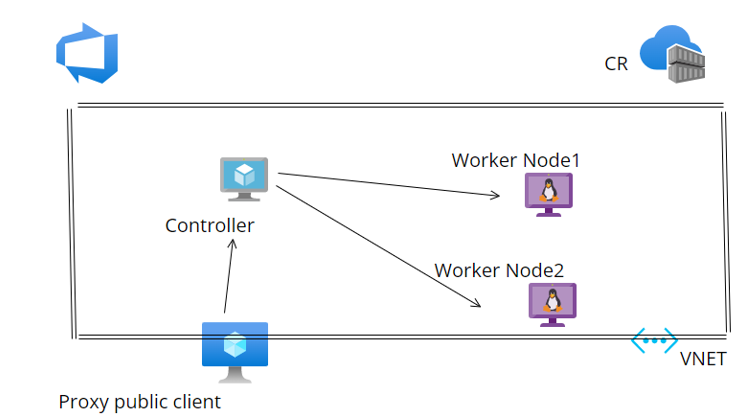
\includegraphics[width = .7\textwidth]{images/k8sdiagram.png}
    \caption{Kubernetes connect to workernodes}        \label{fig:k8sdiagram}
\end{figure}

However, AKS cuts the cost to the absolute minimum since we only need to pay for what we use, namely the worker nodes and the master node is free.
\\\\
K8s provides a rest API that facilitates the interaction with the cluster, once a request is received in the API, typically it's a deployment manifest, then k8s will store a copy of the manifest in the cluster store. Once the store confirms that the transaction is written successfully, then the scheduler will pick the manifest and assign the task to whatever free node is available in the node pool. The task immediately will get an id and it will be registered in the controller in which an event loop is running to check whether the cluster current state meets the desired state registered in the store. On the other side, the worker node has an agent configured as a listener registered in the scheduler once it receives a task it will immediately create a new pod and initialize a suitable runtime for the container to be running. The Kube-proxy job on the worker node is to manage internal networking within the node. See Figure \ref{fig:k8scluster}
\begin{figure}[h]
    \centering
    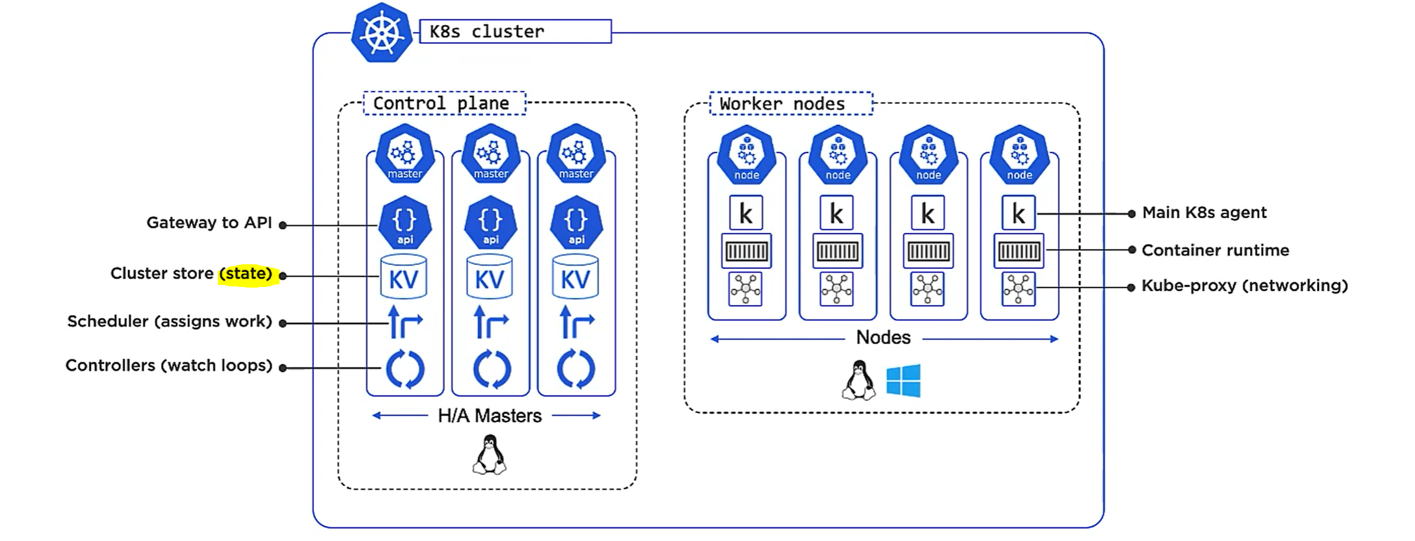
\includegraphics[width = 0.7\textwidth]{k8scluster.png}
    \caption{Kubernetes cluster\cite{https://kubernetes.io/KubernetesKubernetes}}
    \label{fig:k8scluster}
\end{figure}
\\\\
Deployment workflow can be seen in Figure \ref{fig:deploymentWorkflow} and involves the following steps
\begin{enumerate}
    \item Developing the app
    \item Create an image
    \item Store it in an image registry
    \item Create the k8s manifest
    \item Post is to the API server
\end{enumerate} 
\begin{figure}[h]
    \centering
    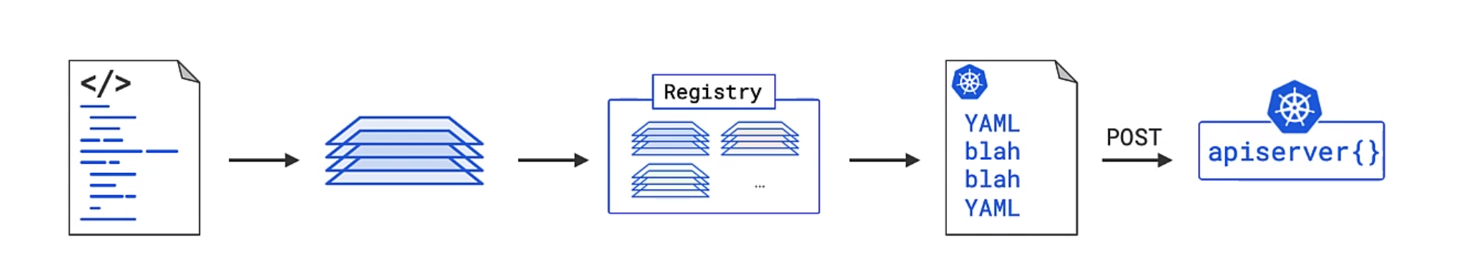
\includegraphics[width = .6\textwidth]{deploymentWorkflow.png}
    \caption{Deployment workflow \cite{https://kubernetes.io/KubernetesKubernetes}}
    \label{fig:deploymentWorkflow}
\end{figure}

MiniTwit infrastructure design: for the MiniTwit AKS setup, the design included two different setups. The first one is a Landing zone infrastructure which is the stateful part of the project, since it contains 1- cosmos database instance running as a service, 2- key vault to store sensitive data like connection string and active client id that allows the pipeline to push images to the CR, 3- container registry for storing docker images. The second one is the AKS cluster itself: the idea is to be able to destroy the entire cluster and rebuild it in no time, since the cluster is a stateless by design, if anything bad happen, security wise for example a malware is installed somewhere in the services, or any other misconfiguration that might happens due to development error, then by running the pipeline we should be able recover to the initial state desired and saved in the pipeline. 

Our cluster consists of the following components; An ingress controller to manage outbound routing into two services which are exposed publicly, namely the simulator and the web application. Behind each service there is exactly one pod running the application inside the container. However, the backend service, which is the busy one, is managing three pods running the spring backend application but not exposed publicly. The Node, shown in Figure \ref{fig:k8s} runs inside a Virtual network which facilitates isolation and works as a Lan network inside the cluster, the gateway for this network is the ingress controller.

\begin{figure}[h]
    \centering
    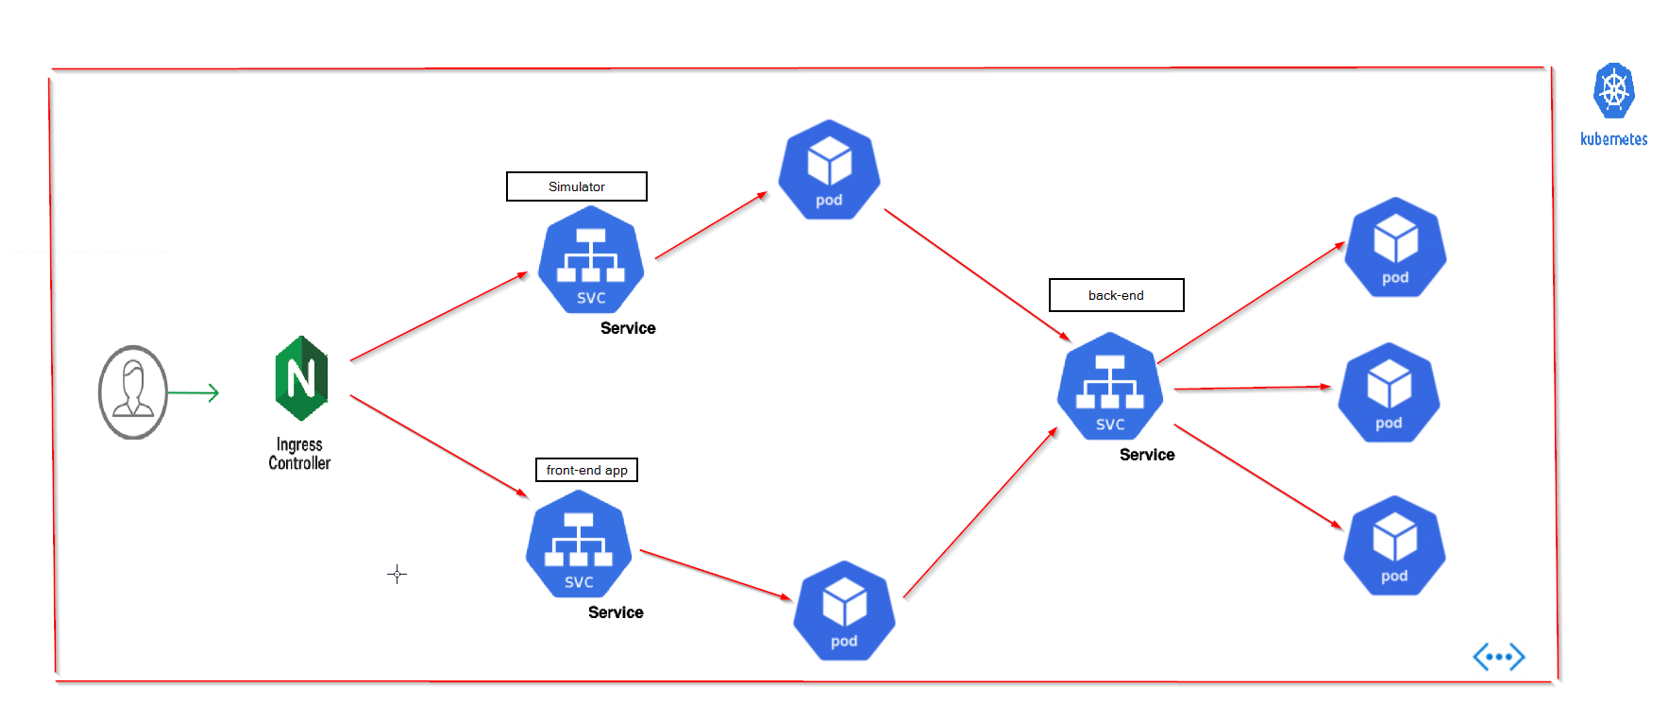
\includegraphics[width = \textwidth]{k8s.png}
    \caption{Kubernetes}
    \label{fig:k8s}
\end{figure}

